\documentclass{standalone}
\usepackage{tikz}
\usetikzlibrary{patterns, positioning}
\usepackage[sfdefault]{ClearSans} %% option 'sfdefault' activates Clear Sans as the default text font
\usepackage[T1]{fontenc}

\begin{document}
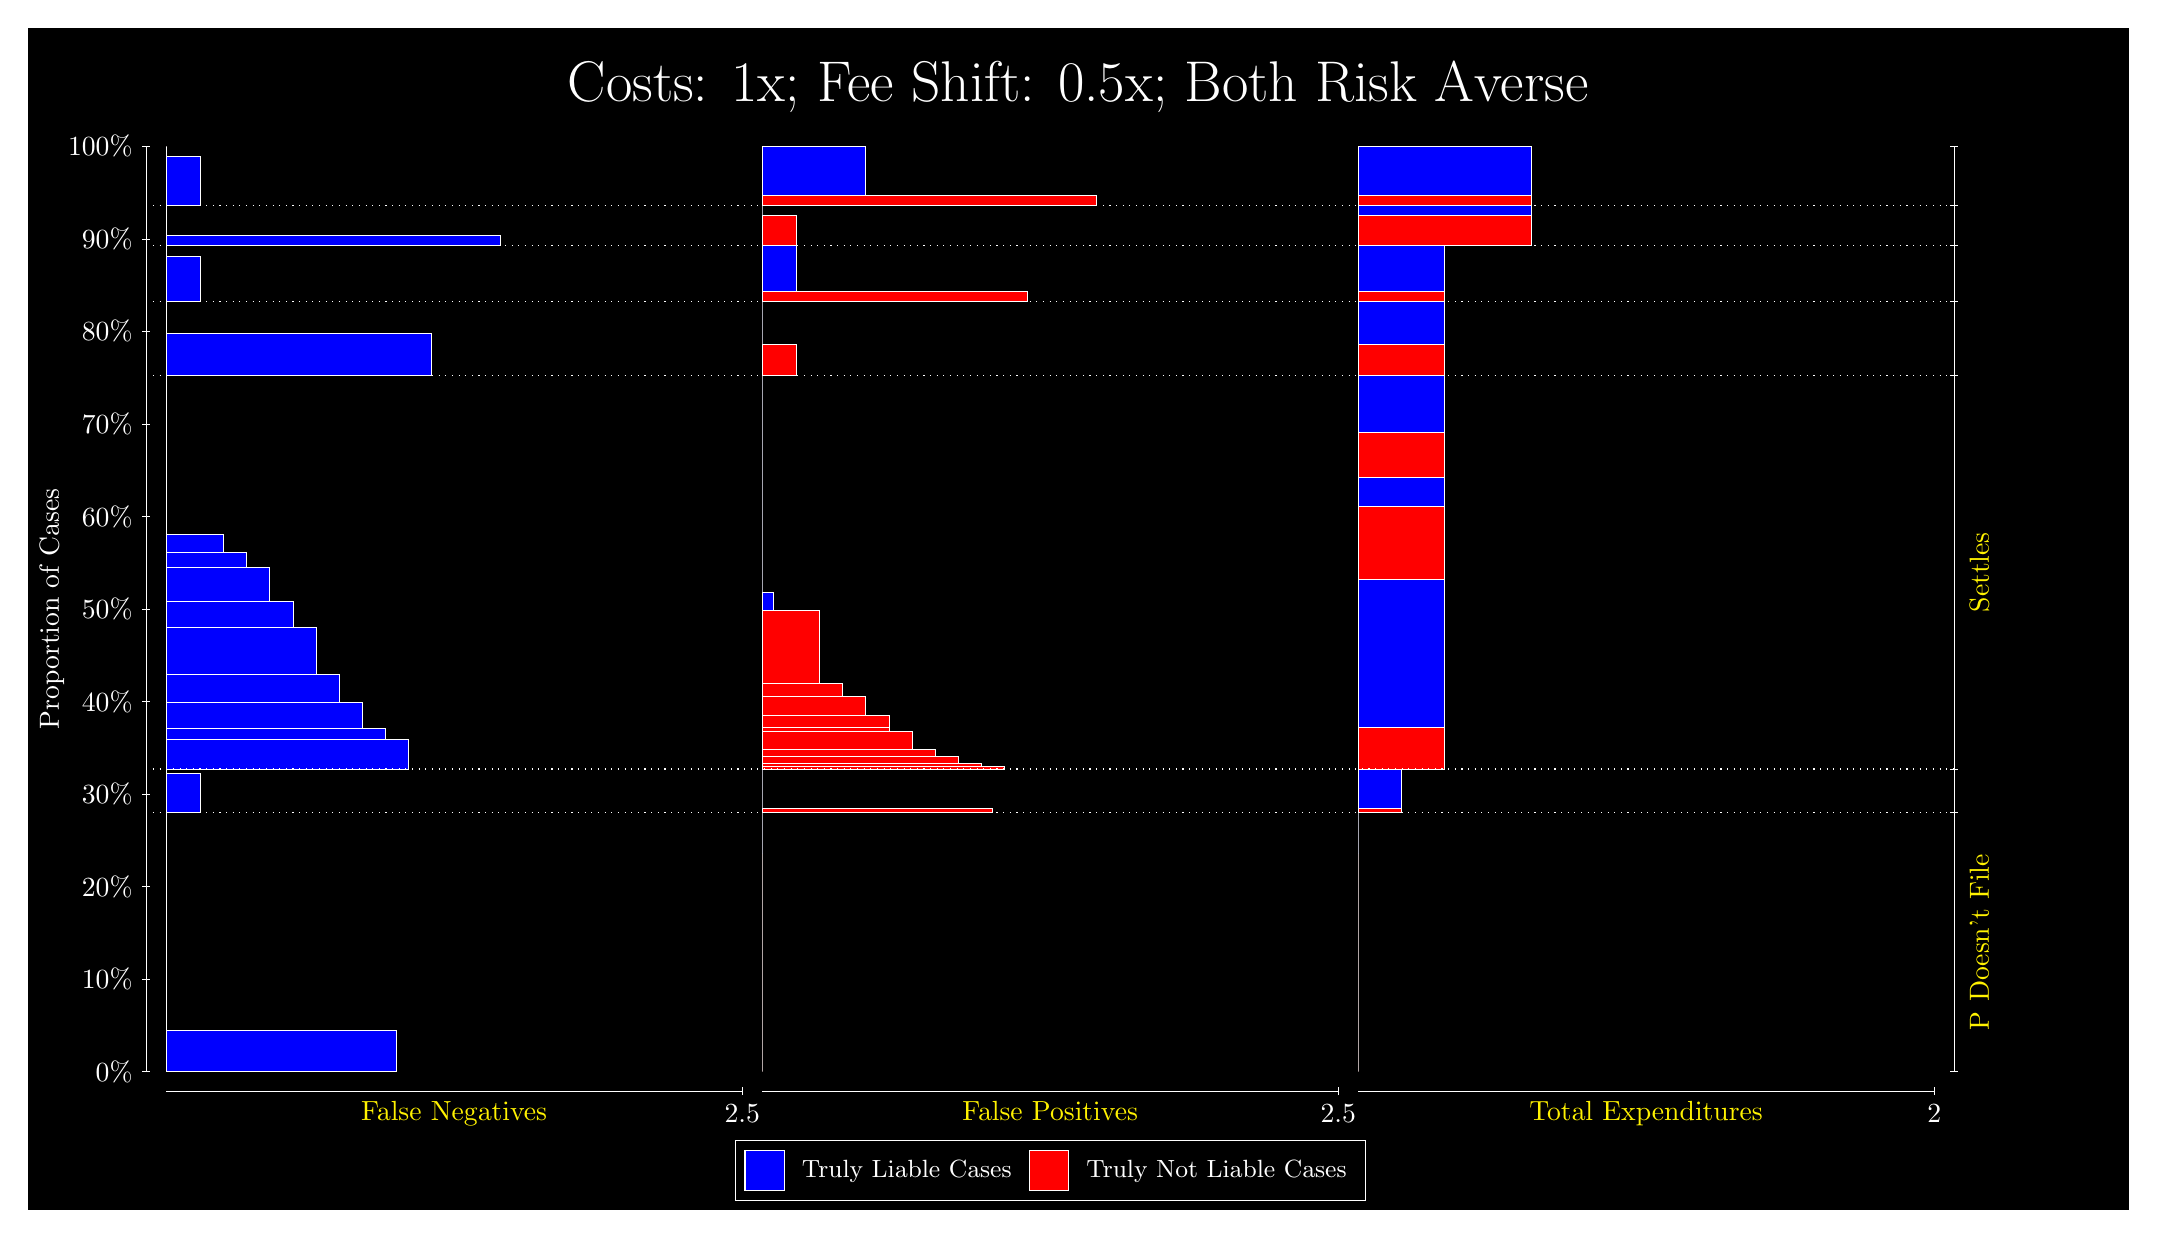
\begin{tikzpicture}
\draw[fill=black] (0,0) rectangle (26.667,15);
\draw[text=white] (0,13.5) rectangle (26.667,15) node[midway] {\huge Costs: 1x; Fee Shift: 0.5x; Both Risk Averse};
\draw[white, very thin] (1.5,1.75) -- (1.5,13.5);
\node[rotate=90, text=white, anchor=center] at (0.3, 7.625) {Proportion of Cases};
\draw[white, very thin] (1.45,1.75) -- (1.55,1.75);
\node[text=white, anchor=east] at (1.45, 1.75) {0\%};
\draw[white, very thin] (1.45,2.925) -- (1.55,2.925);
\node[text=white, anchor=east] at (1.45, 2.925) {10\%};
\draw[white, very thin] (1.45,4.1) -- (1.55,4.1);
\node[text=white, anchor=east] at (1.45, 4.1) {20\%};
\draw[white, very thin] (1.45,5.275) -- (1.55,5.275);
\node[text=white, anchor=east] at (1.45, 5.275) {30\%};
\draw[white, very thin] (1.45,6.45) -- (1.55,6.45);
\node[text=white, anchor=east] at (1.45, 6.45) {40\%};
\draw[white, very thin] (1.45,7.625) -- (1.55,7.625);
\node[text=white, anchor=east] at (1.45, 7.625) {50\%};
\draw[white, very thin] (1.45,8.8) -- (1.55,8.8);
\node[text=white, anchor=east] at (1.45, 8.8) {60\%};
\draw[white, very thin] (1.45,9.975) -- (1.55,9.975);
\node[text=white, anchor=east] at (1.45, 9.975) {70\%};
\draw[white, very thin] (1.45,11.15) -- (1.55,11.15);
\node[text=white, anchor=east] at (1.45, 11.15) {80\%};
\draw[white, very thin] (1.45,12.325) -- (1.55,12.325);
\node[text=white, anchor=east] at (1.45, 12.325) {90\%};
\draw[white, very thin] (1.45,13.5) -- (1.55,13.5);
\node[text=white, anchor=east] at (1.45, 13.5) {100\%};

\draw[white, very thin] (24.457,1.75) -- (24.457,13.5);
\draw[white, very thin] (24.407,1.75) -- (24.507,1.75);
\node[anchor=west] at (24.407, 1.75) {};
\draw[white, very thin] (24.407,5.0371) -- (24.507,5.0371);
\node[anchor=west] at (24.407, 5.0371) {};
\draw[white, very thin] (24.407,5.5917) -- (24.507,5.5917);
\node[anchor=west] at (24.407, 5.5917) {};
\draw[white, very thin] (24.407,10.589) -- (24.507,10.589);
\node[anchor=west] at (24.407, 10.589) {};
\draw[white, very thin] (24.407,11.529) -- (24.507,11.529);
\node[anchor=west] at (24.407, 11.529) {};
\draw[white, very thin] (24.407,12.237) -- (24.507,12.237);
\node[anchor=west] at (24.407, 12.237) {};
\draw[white, very thin] (24.407,12.748) -- (24.507,12.748);
\node[anchor=west] at (24.407, 12.748) {};
\draw[white, very thin] (24.407,13.5) -- (24.507,13.5);
\node[anchor=west] at (24.407, 13.5) {};

\draw[white, very thin, fill=blue] (1.75,1.75) rectangle (4.6775,2.2724);
\draw[white, very thin, fill=red] (1.75,2.2724) rectangle (1.75,5.0371);
\draw[white, very thin, fill=blue] (1.75,5.0371) rectangle (2.1891,5.5374);
\draw[white, very thin, fill=red] (1.75,5.5374) rectangle (1.75,5.5917);
\draw[white, very thin, fill=blue] (1.75,5.5917) rectangle (4.8239,5.9707);
\draw[white, very thin, fill=blue] (1.75,5.9707) rectangle (4.5312,6.1074);
\draw[white, very thin, fill=blue] (1.75,6.1074) rectangle (4.2384,6.4448);
\draw[white, very thin, fill=blue] (1.75,6.4448) rectangle (3.9457,6.795);
\draw[white, very thin, fill=blue] (1.75,6.795) rectangle (3.6529,7.3892);
\draw[white, very thin, fill=blue] (1.75,7.3892) rectangle (3.3602,7.7181);
\draw[white, very thin, fill=blue] (1.75,7.7181) rectangle (3.0674,8.155);
\draw[white, very thin, fill=blue] (1.75,8.155) rectangle (2.7746,8.3429);
\draw[white, very thin, fill=blue] (1.75,8.3429) rectangle (2.4819,8.5769);
\draw[white, very thin, fill=red] (1.75,8.5769) rectangle (1.75,10.589);
\draw[white, very thin, fill=blue] (1.75,10.589) rectangle (5.1167,11.129);
\draw[white, very thin, fill=red] (1.75,11.129) rectangle (1.75,11.529);
\draw[white, very thin, fill=blue] (1.75,11.529) rectangle (2.1891,12.106);
\draw[white, very thin, fill=red] (1.75,12.106) rectangle (1.75,12.237);
\draw[white, very thin, fill=blue] (1.75,12.237) rectangle (5.9949,12.365);
\draw[white, very thin, fill=red] (1.75,12.365) rectangle (1.75,12.748);
\draw[white, very thin, fill=blue] (1.75,12.748) rectangle (2.1891,13.371);
\draw[white, very thin, fill=red] (1.75,13.371) rectangle (1.75,13.5);
\draw[white, very thin, fill=red] (9.3189,1.75) rectangle (9.3189,4.5148);
\draw[white, very thin, fill=blue] (9.3189,4.5148) rectangle (9.3189,5.0371);
\draw[white, very thin, fill=red] (9.3189,5.0371) rectangle (12.246,5.0915);
\draw[white, very thin, fill=blue] (9.3189,5.0915) rectangle (9.3189,5.5917);
\draw[white, very thin, fill=red] (9.3189,5.5917) rectangle (12.393,5.6312);
\draw[white, very thin, fill=red] (9.3189,5.6312) rectangle (12.1,5.6673);
\draw[white, very thin, fill=red] (9.3189,5.6673) rectangle (11.807,5.7526);
\draw[white, very thin, fill=red] (9.3189,5.7526) rectangle (11.515,5.8378);
\draw[white, very thin, fill=red] (9.3189,5.8378) rectangle (11.222,6.0672);
\draw[white, very thin, fill=red] (9.3189,6.0672) rectangle (10.929,6.1196);
\draw[white, very thin, fill=red] (9.3189,6.1196) rectangle (10.929,6.2756);
\draw[white, very thin, fill=red] (9.3189,6.2756) rectangle (10.636,6.5155);
\draw[white, very thin, fill=red] (9.3189,6.5155) rectangle (10.344,6.6858);
\draw[white, very thin, fill=red] (9.3189,6.6858) rectangle (10.051,7.6041);
\draw[white, very thin, fill=blue] (9.3189,7.6041) rectangle (9.4652,7.838);
\draw[white, very thin, fill=blue] (9.3189,7.838) rectangle (9.3189,10.589);
\draw[white, very thin, fill=red] (9.3189,10.589) rectangle (9.758,10.989);
\draw[white, very thin, fill=blue] (9.3189,10.989) rectangle (9.3189,11.529);
\draw[white, very thin, fill=red] (9.3189,11.529) rectangle (12.686,11.661);
\draw[white, very thin, fill=blue] (9.3189,11.661) rectangle (9.758,12.237);
\draw[white, very thin, fill=red] (9.3189,12.237) rectangle (9.758,12.62);
\draw[white, very thin, fill=blue] (9.3189,12.62) rectangle (9.3189,12.748);
\draw[white, very thin, fill=red] (9.3189,12.748) rectangle (13.564,12.877);
\draw[white, very thin, fill=blue] (9.3189,12.877) rectangle (10.636,13.5);
\draw[white, very thin, fill=red] (16.888,1.75) rectangle (16.888,4.5148);
\draw[white, very thin, fill=blue] (16.888,4.5148) rectangle (16.888,5.0371);
\draw[white, very thin, fill=red] (16.888,5.0371) rectangle (17.437,5.0915);
\draw[white, very thin, fill=blue] (16.888,5.0915) rectangle (17.437,5.5917);
\draw[white, very thin, fill=red] (16.888,5.5917) rectangle (17.986,6.1196);
\draw[white, very thin, fill=blue] (16.888,6.1196) rectangle (17.986,8.0041);
\draw[white, very thin, fill=red] (16.888,8.0041) rectangle (17.986,8.9224);
\draw[white, very thin, fill=blue] (16.888,8.9224) rectangle (17.986,9.3014);
\draw[white, very thin, fill=red] (16.888,9.3014) rectangle (17.986,9.8675);
\draw[white, very thin, fill=blue] (16.888,9.8675) rectangle (17.986,10.589);
\draw[white, very thin, fill=red] (16.888,10.589) rectangle (17.986,10.989);
\draw[white, very thin, fill=blue] (16.888,10.989) rectangle (17.986,11.529);
\draw[white, very thin, fill=red] (16.888,11.529) rectangle (17.986,11.661);
\draw[white, very thin, fill=blue] (16.888,11.661) rectangle (17.986,12.237);
\draw[white, very thin, fill=red] (16.888,12.237) rectangle (19.083,12.62);
\draw[white, very thin, fill=blue] (16.888,12.62) rectangle (19.083,12.748);
\draw[white, very thin, fill=red] (16.888,12.748) rectangle (19.083,12.877);
\draw[white, very thin, fill=blue] (16.888,12.877) rectangle (19.083,13.5);
\draw[white, dotted] (1.5,5.0371) -- (24.457,5.0371);
\draw[white, dotted] (1.5,5.5917) -- (24.457,5.5917);
\draw[white, dotted] (1.5,10.589) -- (24.457,10.589);
\draw[white, dotted] (1.5,11.529) -- (24.457,11.529);
\draw[white, dotted] (1.5,12.237) -- (24.457,12.237);
\draw[white, dotted] (1.5,12.748) -- (24.457,12.748);
\draw[white, very thin] (1.75,1.5) -- (9.0689,1.5);
\node[text=yellow, anchor=north] at (5.4094, 1.5) {False Negatives};
\draw[white, very thin] (9.0689,1.45) -- (9.0689,1.55);
\node[text=white, anchor=north] at (9.0689, 1.45) {2.5};

\draw[white, very thin] (9.3189,1.5) -- (16.638,1.5);
\node[text=yellow, anchor=north] at (12.978, 1.5) {False Positives};
\draw[white, very thin] (16.638,1.45) -- (16.638,1.55);
\node[text=white, anchor=north] at (16.638, 1.45) {2.5};

\draw[white, very thin] (16.888,1.5) -- (24.207,1.5);
\node[text=yellow, anchor=north] at (20.547, 1.5) {Total Expenditures};
\draw[white, very thin] (24.207,1.45) -- (24.207,1.55);
\node[text=white, anchor=north] at (24.207, 1.45) {2};

\node[text=yellow, centered, rotate=90] at (24.777, 3.3936) {P Doesn't File};

\node[text=yellow, centered, rotate=90] at (24.777, 8.0905) {Settles};





\draw (12.978300999999998,1.5) node[draw=none] (baseCoordinate) {};
\begin{scope}[align=center]
        \matrix[scale=0.5, draw=white, below=0.5cm of baseCoordinate, nodes={draw}, column sep=0.1cm]{
            \node[rectangle, draw, minimum width=0.5cm, minimum height=0.5cm, fill=blue] {}; &
            \node[draw=none, font=\small, text=white] (B) {Truly Liable Cases}; &
            \node[rectangle, draw, minimum width=0.5cm, minimum height=0.5cm, fill=red] {}; &
            \node[draw=none, font=\small, text=white] (B) {Truly Not Liable Cases}; \\
            };
\end{scope}

\end{tikzpicture}
\end{document}